% !TEX encoding = UTF-8 Unicode
% !TEX root = Simulation.tex

%%%  This is the main driver file.   It is mostly a list of file includes.   Read through and edit as needed.

\documentclass[table]{book}

\input{paperstyle.tex} % This sets the format.

% Add your title page contents here 
\title{{ \rule{\linewidth}{0.5mm}}\\[2mm] {\huge \bfseries  Simulation }\\[-1mm] {\rule{\linewidth}{0.5mm}} \\  \vfill
{\LARGE \bfseries  Natural Computing Homework }\vfill}
\author{Paul Blasi  }
\date{\today}


\begin{document}

\frontmatter

% Comment out items you don't need

\addcontentsline{toc}{chapter}{Title}
\maketitle
\tableofcontents
\addcontentsline{toc}{chapter}{Contents}
\listoffigures
\addcontentsline{toc}{chapter}{List of Figures}
\listoftables
\addcontentsline{toc}{chapter}{List of Tables}
\listofalgorithms
\addcontentsline{toc}{chapter}{List of Algorithms}

\chapter{Document Preparation and Updates}
% !TEX root = Simulation.tex



Current Version [1.1.0]
\vspace*{5mm}

{\color{MSBlue3}
\noindent
\textit{Prepared By:}\\
\textit{Paul Blasi}\\
}

\vfill
\noindent
{\color{color02} \textit{\textbf{Revision History}}}\\
\begin{tabular}{|>{\raggedright}p{1.5cm}|>{\raggedright}p{3cm}|>{\raggedright}p{1.5cm}|>{\raggedright}p{9cm}|}
\hline
\textit{\textbf{Date}} &  \textit{\textbf{Author}} & \textit{\textbf{Version}} & \textit{\textbf{Comments}}\tabularnewline
\hline
 \textit{\textbf{4/29/15}} & \textit{Paul Blasi} & \textit{1.0.0} & \textit{Wrote down problem set.}\tabularnewline
\hline
\textit{\textbf{4/29/15}} & \textit{Paul Blasi} & \textit{1.1.0} & \textit{Finished Chapter 9 Problems}\tabularnewline
\hline
\textit{\textbf{4/30/15}} & \textit{Paul Blasi} & \textit{1.1.0} & \textit{Finished 7.10 \& 7.15}\tabularnewline
\hline
\end{tabular}
\vfill


 
 % Core content to follow ...
 
\mainmatter

%%  Add to the following chapters
% you may also need additional chapters ...

% !TEX root = Simulation.tex

\chapter{Fractals - Text Chapter 7}

\section{Problem 10}
\textbf{
Implement a bracketed OL-system and reproduce all plant-like structures of Figure~7.24 in the text. Change some derivation rules and see what happens. Make your own portfolio with at least ten plants.
}

\hfill \\

The first step to solving this problem was to gather the necessary test input. The parameters from Figure~7.24 in the text were summarized into Figure~\ref{7.24_rep}. The images were created using the program developed for the problem.

After collecting the necessary data, I saw two distinct parts to this problem. One was to create the L-system strings, and the other was to interpret them using Python's Turtle graphics (as suggested).

\subsection{L-system generation}
L-systems are rather straight forward so I made a simple class to encapsulate them. I tested this class against the example in section 7.4.3 in the text. The code can be found in Listing~\ref{LSystem.py} and the results can be found in Figure~\ref{lsystem_results}.

\begin{figure}
\centering
\includegraphics[scale=.75]{LSystemResults}
\caption{LSystem Results}
\label{lsystem_results}
\end{figure}


\subsection{Turtle Graphics representation}
Generating the actual Python turtle code was also simple. I encapsulated the process in a class called LSystemTurtle that would initialize, run, and save the results from each L-system. This code can be found in Listing~\ref{LSystemTurtle.py}. The default function run if this python file is run generated the six example images seen in Figure~\ref{7.24_rep}. It's worth noting that even with the turtle speed set to 0 (meaning no animation), these plants took a very long time to reproduce\footnote{Like, "I could have grown a real tree faster than this" very long time}.

After generating the given examples the task was to mess with the parameters to create a portfolio of ten different plants. Below I'll list my thought processes for each of the plants in the portfolio found in Appendix~\ref{plant_portfolio}. For the last two, I had to modify my code slightly. The modification amounted to checking if the d and delta variables were functions and if they were calling them instead of using them as normal. You can see this around lines 24, 40, and 45 in the code. The code to actually create the portfolio can be seen in Listing~\ref{PlantPortfolio.py}.

\subsubsection{Symmetrical G}
For this plant, I decided to keep the $F \rightarrow FF$ parameter and just adapt the $G$ parameter. I like symmetry so my thought was to make a string that is a palindrome and use that as the replacement in G. The full set of parameters I decided to go with was:

\begin{center}
$\begin{aligned}
& t = 4, \delta = 22.5\degree \\
& \omega = G \\
& G \rightarrow GG+[GF-][-FG]+GG
& F \rightarrow FF
\end{aligned}$
\end{center}

\subsubsection{Symmetrical G with +/- swapping}
For this plant, I kept the same parameters as the previous one, but instead of being a true palindrome, I swapped the + and - signs on the second half of the G parameter. This gave me:

\begin{center}
$\begin{aligned}
& t = 4, \delta = 22.5\degree \\
& \omega = G \\
& G \rightarrow GG+[GF-][+FG]-GG
& F \rightarrow FF
\end{aligned}$
\end{center}

\subsubsection{Symmetrical F only}
In this parameter set, I removed the G parameter and went with only one parameter to choose from. Again, I wanted to experiment with symmetry so I went with a palindrome.

\begin{center}
$\begin{aligned}
& t = 4, \delta = 22.5\degree \\
& \omega = 'F' \\
& F \rightarrow FF+[-F[--F][F--]F-]+FF
\end{aligned}$
\end{center}

\subsubsection{Symmetrical F only with +/- swapping}
This time I used the same single parameter set as the previous plant but swapped the + and - signs in the second half of the palindrome.

\begin{center}
$\begin{aligned}
& t = 4, \delta = 22.5\degree \\
& \omega = 'F' \\
& F \rightarrow FF+[-F[--F][F++]F+]-FF
\end{aligned}$
\end{center}

\subsubsection{Turning F}
For this plant I wanted to make a very asymmetrical plant. My plan for this was to have the F parameter constantly turn in one direction. This plant is directly modified from the plant in Figure~\ref{7.24_rep}(c).

\begin{center}
$\begin{aligned}
& t = 4, \delta = 22.5\degree \\
& \omega = G \\
& G \rightarrow F[+FFG][G]-FG \\
& F \rightarrow FF-FFF
\end{aligned}$
\end{center}

\subsubsection{Symmetrical Turning F}
This time I wanted to try having a palindrome with turns for the F value. This one is again adapted from Figure~\ref{7.24_rep}(c).

\begin{center}
$\begin{aligned}
& t = 4, \delta = 22.5\degree \\
& \omega = G \\
& G \rightarrow F[+FFG][G]-FG \\
& F \rightarrow FF-F-FF
\end{aligned}$
\end{center}

\subsubsection{Symmetrical Turning F with +/- swapping}
This one is adapted from the above plant with the second - sign being replaced with a +. The hope was that this would produce a "wavy" plant.

\begin{center}
$\begin{aligned}
& t = 4, \delta = 22.5\degree \\
& \omega = G \\
& G \rightarrow F[+FFG][G]-FG \\
& F \rightarrow FF-F+FF
\end{aligned}$
\end{center}

\subsubsection{Similar G \& F}
For this plant, I wanted to see what happens when F and G are similar, but with the Fs and Gs in them swapped.

\begin{center}
$\begin{aligned}
& t = 4, \delta = 22.5\degree \\
& \omega = G \\
& G \rightarrow FF-G[+GF]G \\
& F \rightarrow GG-F[+FG]F
\end{aligned}$
\end{center}

\subsubsection{Randomized distance}
In an attempt to get a random plant, I decided to make the distance stepped at each point be determined randomly. The other parameters where taken from Figure~\ref{7.24_rep}(b).

\begin{center}
$\begin{aligned}
& t = 4, \delta = 22.5\degree \\
& \omega = F \\
& F \rightarrow FF+[+F-F-F]-[-F+F+F]
\end{aligned}$
\end{center}

\subsubsection{Randomized turn ($\delta$)}
In another attempt to get a random plant, I decided to make the angle turned at each point be determined randomly. The other parameters where taken from Figure~\ref{7.24_rep}(b).

\begin{center}
$\begin{aligned}
& t = 4, \delta_i = random_i(20.0, 30.0) \\
& \omega = F \\
& F \rightarrow FF+[+F-F-F]-[-F+F+F]
\end{aligned}$
\end{center}

\begin{figure}
\centering
\begingroup \everymath{\scriptsize} \setlength{\medmuskip}{0mu}
\begin{tabular}{ | c | c | c | }
\hline
%\includegraphics[width=.3\linewidth]{LSystemExamples/lsystem_a} &
%\includegraphics[width=.3\linewidth]{LSystemExamples/lsystem_b} &
%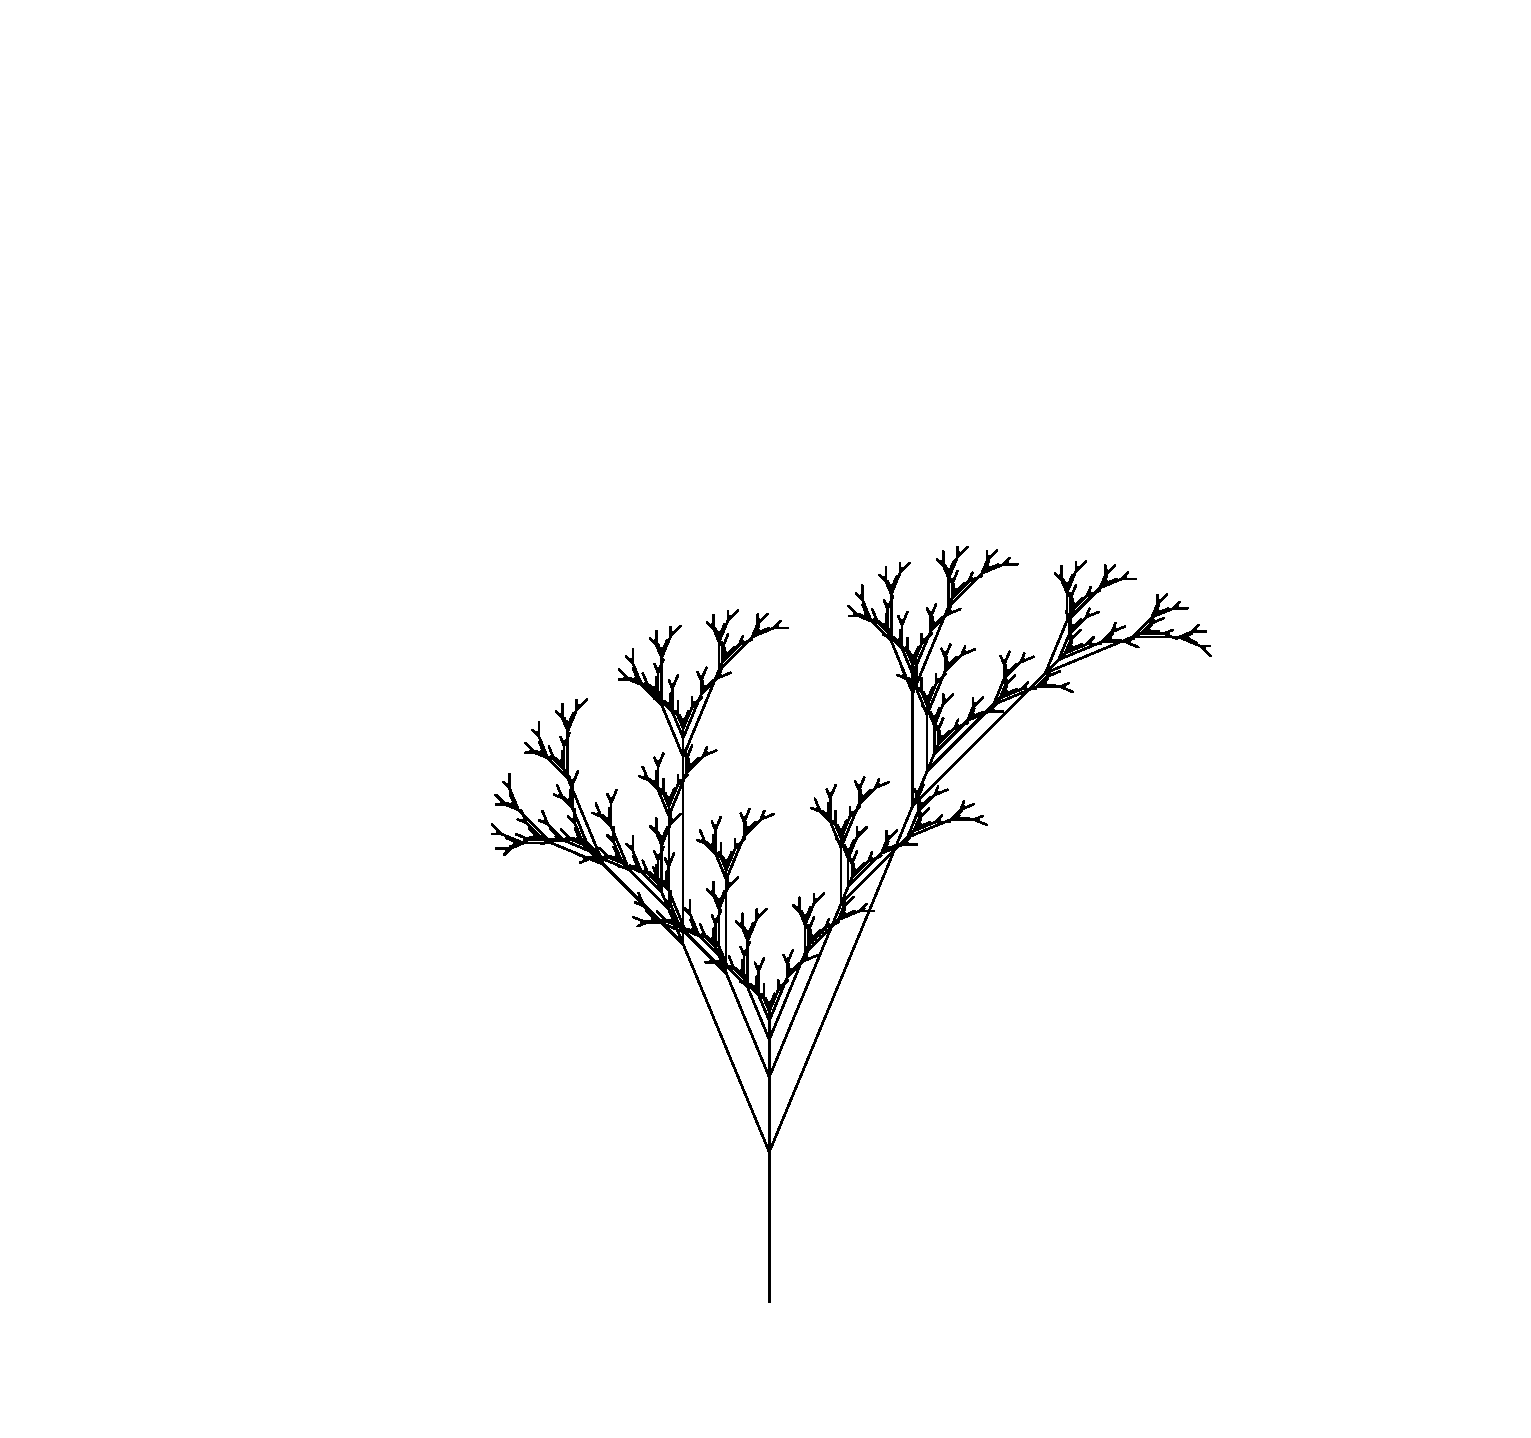
\includegraphics[width=.3\linewidth]{LSystemExamples/lsystem_c} \\

$\begin{aligned}
& t = 8, \delta = 22.5\degree \\
& \omega = G \\
& G \rightarrow F+[[G]-G]-F[-FG]+G \\
& F \rightarrow FF
\end{aligned}$ & 
$\begin{aligned}
& t = 4, \delta = 22.5\degree \\
& \omega = F \\
& F \rightarrow FF+[+F-F-F]-[-F+F+F]
\end{aligned}$ & 
$\begin{aligned}
& t = 6, \delta = 22.5\degree \\
& \omega = G \\
& G \rightarrow F[+FFG][G]-FG \\
& F \rightarrow FF
\end{aligned}$ \\ \hline

%\includegraphics[width=.3\linewidth]{LSystemExamples/lsystem_d} &
%\includegraphics[width=.3\linewidth]{LSystemExamples/lsystem_e} &
%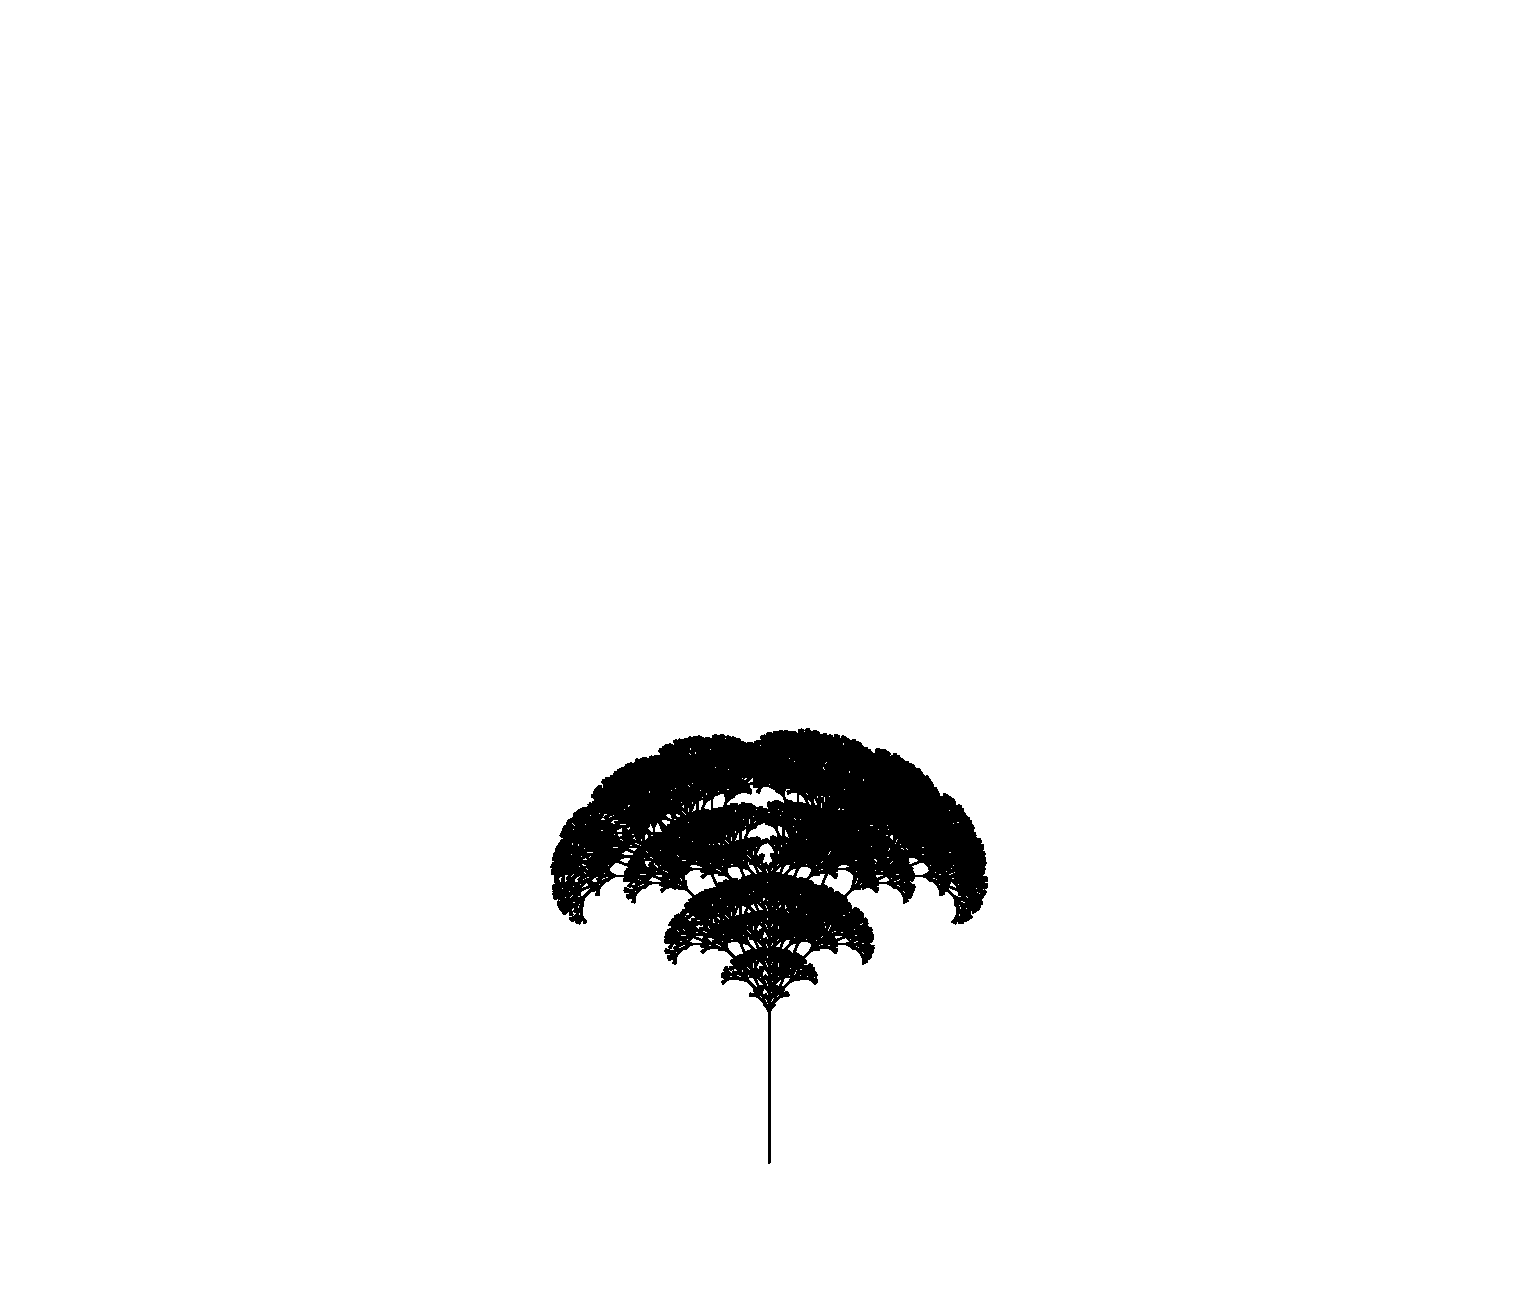
\includegraphics[width=.3\linewidth]{LSystemExamples/lsystem_f} \\

$\begin{aligned}
& t = 9, \delta = 20\degree \\
& \omega = G \\
& G \rightarrow F[-G]F[+G]-G \\
& F \rightarrow FF
\end{aligned}$ &
$\begin{aligned}
& t = 9, \delta = 25.7\degree \\
& \omega = G \\
& G \rightarrow F[-G][+G]FG \\
& F \rightarrow FF
\end{aligned}$ &
$\begin{aligned}
& t = 5, \delta = 22.5\degree \\
& \omega = G \\
& G \rightarrow FG[-F[G]-G][G+G][+F[G]+G] \\
& F \rightarrow FF
\end{aligned}$ \\ \hline
\end{tabular}
\endgroup
\caption{Reproduction of figure 7.24 in the text}
\label{7.24_rep}
\end{figure}

\section{Problem 15}
\textbf{
Implement a random iterated function system (RIFS) to generate all the fractals whose codes are presented in Table~7.3 in the text.
}

\hfill \\

Again, the first step was to reproduce the data needed for the problem. Table~7.3 from the text has been reproduced in Table~\ref{7.3_rep}.

With this data available I created a simple class to do the iterated functions, which would output a list of x and y values that I would plot after the full set was created. This is a slight (less graphics intensive) modification of Algorithm~7.3 in the text. This code can be seen in Listing~\ref{RIFS.py}. The resulting fractals can be seen in Appendix~\ref{RIFS_results}.

\begin{table}
\begin{tabular}{ c c }
	\begin{tabular}{ c c c c c c c c }
	\hline
	w & a & b & c & d\footnote{Corrected as suggested on assignment page} & e & f & p \\
	\hline
	1 & 0.5 & 0 & 0 & 0.5 & 1 & 1 & 0.33 \\
	2 & 0.5 & 0 & 0 & 0.5 & 1 & 50 & 0.33 \\
	3 & 0.5 & 0 & 0 & 0.5 & 50 & 50 & 0.34 \\
	\hline
	\multicolumn{8}{c}{Sierpinski Gasket}
	\end{tabular} &

	\begin{tabular}{ c c c c c c c c }
	\hline
	w & a & b & c & d & e & f & p \\
	\hline
	1 & 0.5 & 0 & 0 & 0.5 & 1 & 1 & 0.25 \\
	2 & 0.5 & 0 & 0 & 0.5 & 50 & 1 & 0.25 \\
	3 & 0.5 & 0 & 0 & 0.5 & 1 & 50 & 0.25 \\
	4 & 0.5 & 0 & 0 & 0.5 & 50 & 50 & 0.25 \\
	\hline
	\multicolumn{8}{c}{Square}
	\end{tabular} \\
	
	\hfill & \hfill \\
	
	\begin{tabular}{ c c c c c c c c }
	\hline
	w & a & b & c & d & e & f & p \\
	\hline
	1 & 0 & 0 & 0 & 0.16 & 0 & 0 & 0.01 \\
	2 & 0.85 & 0.04 & -0.04 & 0.85 & 0 & 1.6 &0.85 \\
	3 & 0.2 & -0.26 & 0.23 & 0.22 & 0 & 1.6 & 0.07 \\
	4 & -0.15 & 0.28 & 0.26 & 0.24 & 0 & 0.44 & 0.07 \\
	\hline
	\multicolumn{8}{c}{Barnsley Fern}
	\end{tabular} &
	
	\begin{tabular}{ c c c c c c c c }
	\hline
	w & a & b & c & d & e & f & p \\
	\hline
	1 & 0 & 0 & 0 & 0.5 & 0 & 0 & 0.05 \\
	2 & 0.42 & -0.42 & 0.42 & 0.42 & 0 & 0.2 & 0.40 \\
	3 & 0.42 & 0.42 & -0.42 & 0.42 & 0 & 0.2 & 0.40 \\
	4 & 0.1 & 0 & 0 & 0.1 & 0 & 0.2 & 0.15 \\
	\hline
	\multicolumn{8}{c}{Tree}
	\end{tabular}
\end{tabular}
\caption{Reproduction of Table 7.3 from the text}
\label{7.3_rep}
\end{table}

\section{Problem 21}
\textbf{
Implement the random midpoint displacement algorithm in 3D and generate some fractal landscapes. Study the influence of H on the landscapes generated.
}

\hfill \\

% !TEX root = Simulation.tex

\chapter{Cellular Automata - Chapter 7}

\section{Problem 1 (from slides)}
\textbf{
Modify the heat flow example to deal with insulated conditions on the top and bottom boundary. Insulation means zero flux or u[N][j] = u[N-1][j]. This implies that instead of fixed valued ghost points on the top and bottom, you modify the CA rule using the previous relation.
}

\hfill \\

\section{Problem 2 (from slides)}
\textbf{
Reproduce patterns theta, lambda, mu, and alpha in the Gray-Scott Model CA. You don't need to follow their color scheme.
}

\hfill \\

% !TEX root = Simulation.tex

\chapter{ALife - Text Chapter 8}

\section{Problem 3}
\textbf{
Choose one of the sample projects of StarLogo and solve its exploration tasks (\url{http://education.mit.edu/starlogo/projects.html}). Write a brief report with the results obtained including any theoretical background knowledge that may eventually be necessary to perform the exploration.
}

\hfill \\

Unfortunately, I got sidetracked with attempting to speed up the python for the Gray-Scott models and didn't leave myself enough time to finish this problem. I may play with the projects at some point in the future anyway as they look very interesting. Specifically the Turtle Graphics and the Fireflies projects looked interesting to me.


\section{Problem 4}
\textbf{
Implement a bi-dimensional CA following the rules of 'The Game of Life'.
}

\hfill \\

This was a rather straight-forward problem. I gathered the rules from Wikipedia and went to work. The hardest part was making a UI with Tkinter. I created a subclass of Canvas to display rectangles on the screen and tied those rectangles up to click events so that the board could be initialized by the user. After that implementing the CA and the start/pause and clear buttons was simple. I tested the application with the Gosper Glider Gun and a couple other small repeating patterns because they were easy to see if it was working. A couple states for the Gosper Glider Gun can be seen in Figure~\ref{gosper}.

Code for this problem can be found in Listing~\ref{GameOfLife.py}.

\begin{figure}
\centering
\begin{tabular}{c c c}
\includegraphics[width=.3\textwidth]{CAs/gosper_1} &
\includegraphics[width=.3\textwidth]{CAs/gosper_2} &
\includegraphics[width=.3\textwidth]{CAs/gosper_3} \\

(a) & (b) & (c) \\
\end{tabular}
\caption{States of the Gosper Glider Gun: (a) Initial state, (b) rebound, (c) near initial with glider}
\label{gosper}
\end{figure}

% !TEX root = Simulation.tex

\chapter{DNA Computing - Text Chapter 9}

Most of this section of the assignment was paraphrased or expanded on from Wikipedia articles.

\section{Problem 1}
\textbf{
Name four problems that cannot be solved by a Turing machine.
}

\hfill \\

\begin{description}
\item Halting Problem
\item Determining a busy beaver\footnote{"Busy Beaver" is my favorite program name of all time.} champion
\item The Mortality Problem
\item Determining whether a given machine computes a partial function with a nontrivial property of partial functions.
\end{description}


\section{Problem 2}
\textbf{
Name four NP-complete and four NP-hard problems.
}

\hfill \\

\begin{minipage}[b]{.5\hsize}
	\centerline{\textbf{NP-complete problems}}
	\begin{description}
	\item{SAT problem}
	\item{Hamiltonian Path Problem (HPP)}
	\item{Knapsack Problem}
	\item{Partition Problem}
	\end{description}
\end{minipage}	
\begin{minipage}[b]{.5\hsize}
	\centerline{\textbf{NP-hard problems}}
	\begin{description}
	\item{Subset Sum Problem}
	\item{Traveling Salesman Problem}
	\item{K Minimum-spanning tree}
	\item{Graph Coloring Problem}
	\end{description}
\end{minipage}


\newpage
\section{Problem 5}
\textbf{
The two most basic DNA sequencing techniques are known as a) Maxam-Gilbert and b) Sanger, after their proponents. Explain how each of these techniques work and contrast them.
}

\hfill \\

\begin{description}
\item{\textbf{Maxam-Gilbert Sequencing}} \hfill \\
Maxam-Gilbert Sequencing works by cleaving the DNA strands via four different solutions. The solutions are balanced in such a way that each strand will, on average, only be cleaved once. The four solutions cleave at different deoxynucleotides: (A + G), G, C, \& (C + T).

After electrophoresing the leftover strands to sort them by size, you are left with a distribution of sizes in each solution. Reading these from shortest to longest, you can infer the deoxynucleotide at that position. Note: in the case of the (A + G) and (C + T) bands, the presence of A and T are infered by that band showing and a lack of the G and C bands respectively. An example graphic of Maxam-Gilbert Sequencing can be seen in Figure~\ref{sequencing} (a).

\item{\textbf{Sanger Sequencing}} \hfill \\
Sanger Sequencing clones a sequence of DNA in four different solutions. Each solution contains 3 of the normal deoxynucleotides that make up DNA chains. The fourth deoxynucleotide is replaced with a corresponding \textit{di}-deoxynucleotide which inhibits chaining due to it's lack of a 3'-OH group used to form phosphodiester bonds. The di-deoxynucleotides can be labeled through various methods including florescence or radioactivity.

Once the DNA is copied, the four strands are heat denatured and separated by length using gel electrophoresis. The length of the strands was limited by the di-deoxynucleotide which means the different lengths of the strands in each solution corresponds to places where the corresponding deoxynucleotide would reside. The sequence can then be read by reading the relative positions in the four lanes. An example of this type of sequencing can be found in Figure~\ref{sequencing} (b).

\end{description}

\begin{figure} 
\centering
\begin{tabular}{ c c c }
\includegraphics[scale=.75]{MaxamGilbertSequencing} & \hspace{10pt} &
\includegraphics{SangerSequencing} \\
(a) &  & (b)
\end{tabular}
\caption[DNA Sequencing Methods]{DNA Sequencing Methods. (a)Maxam-Gilbert Sequencing (b)Sanger Sequencing}
\label{sequencing}
\end{figure}




%%%  Done with chapters
% Bib stuff

\bibliographystyle{plain}
\bibliography{refs.bib}
\addcontentsline{toc}{chapter}{Bibliography}



% In our style file, appendices are numbered with capital letters
\appendix

\chapter{Supporting Materials}
\section{Plant Portfolio} \label{plant_portfolio}
\begin{tabular}{ c c }
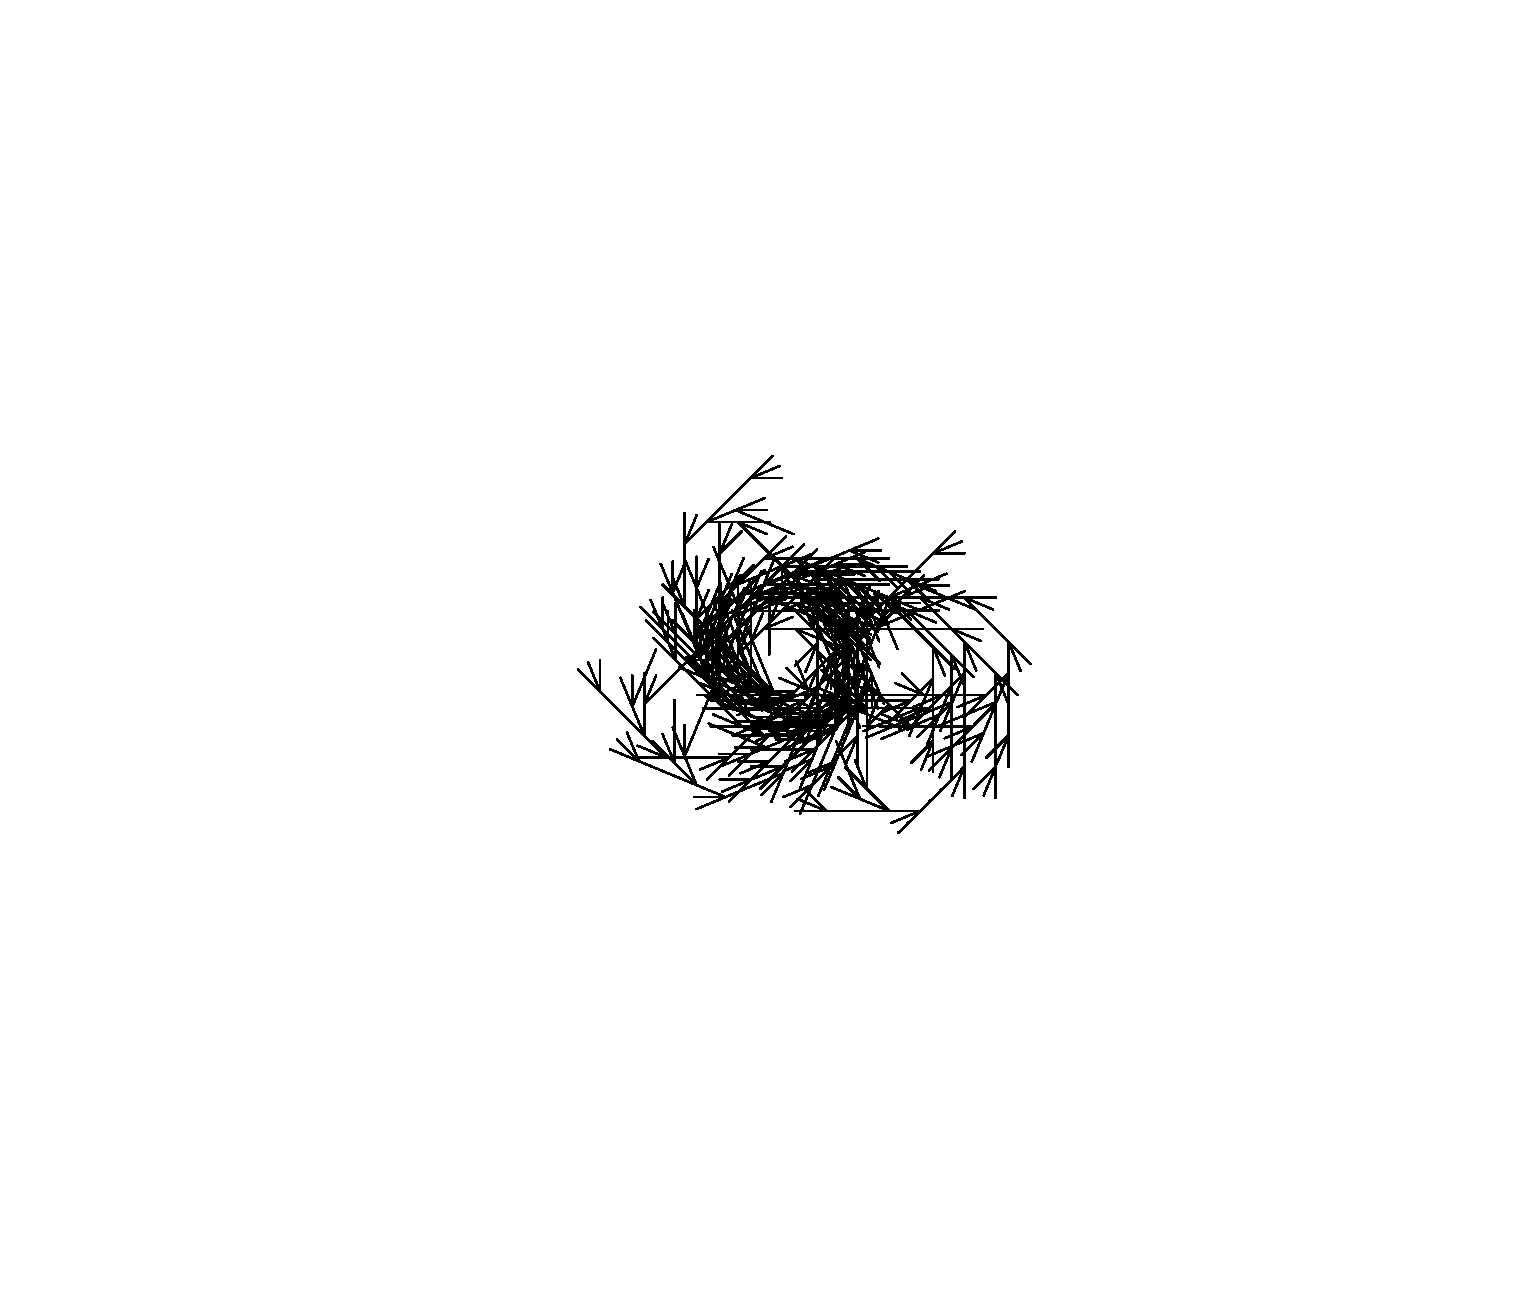
\includegraphics[width=.5\textwidth]{LSystem/plant_1} &
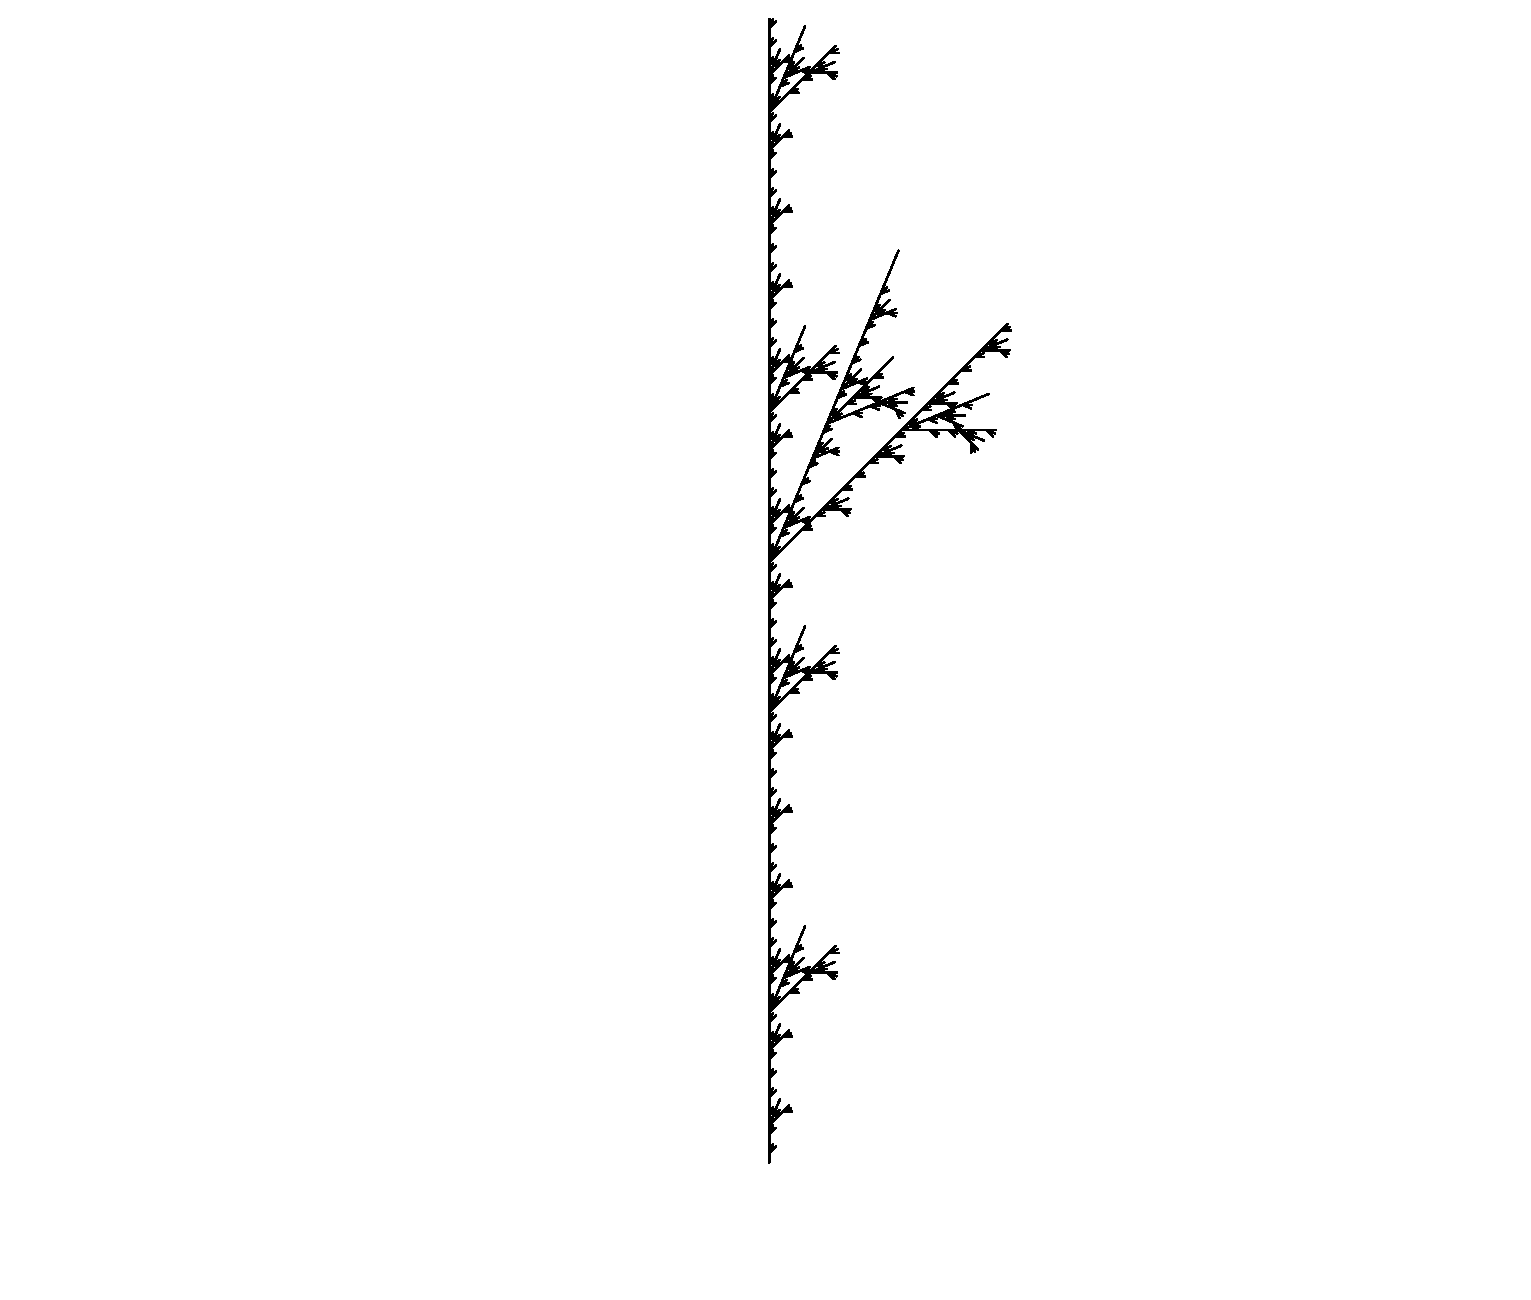
\includegraphics[width=.5\textwidth]{LSystem/plant_2} \\
Symmetrical G & Symmetrical G with +/- swapping \\


\includegraphics[width=.5\textwidth]{LSystem/plant_3} &
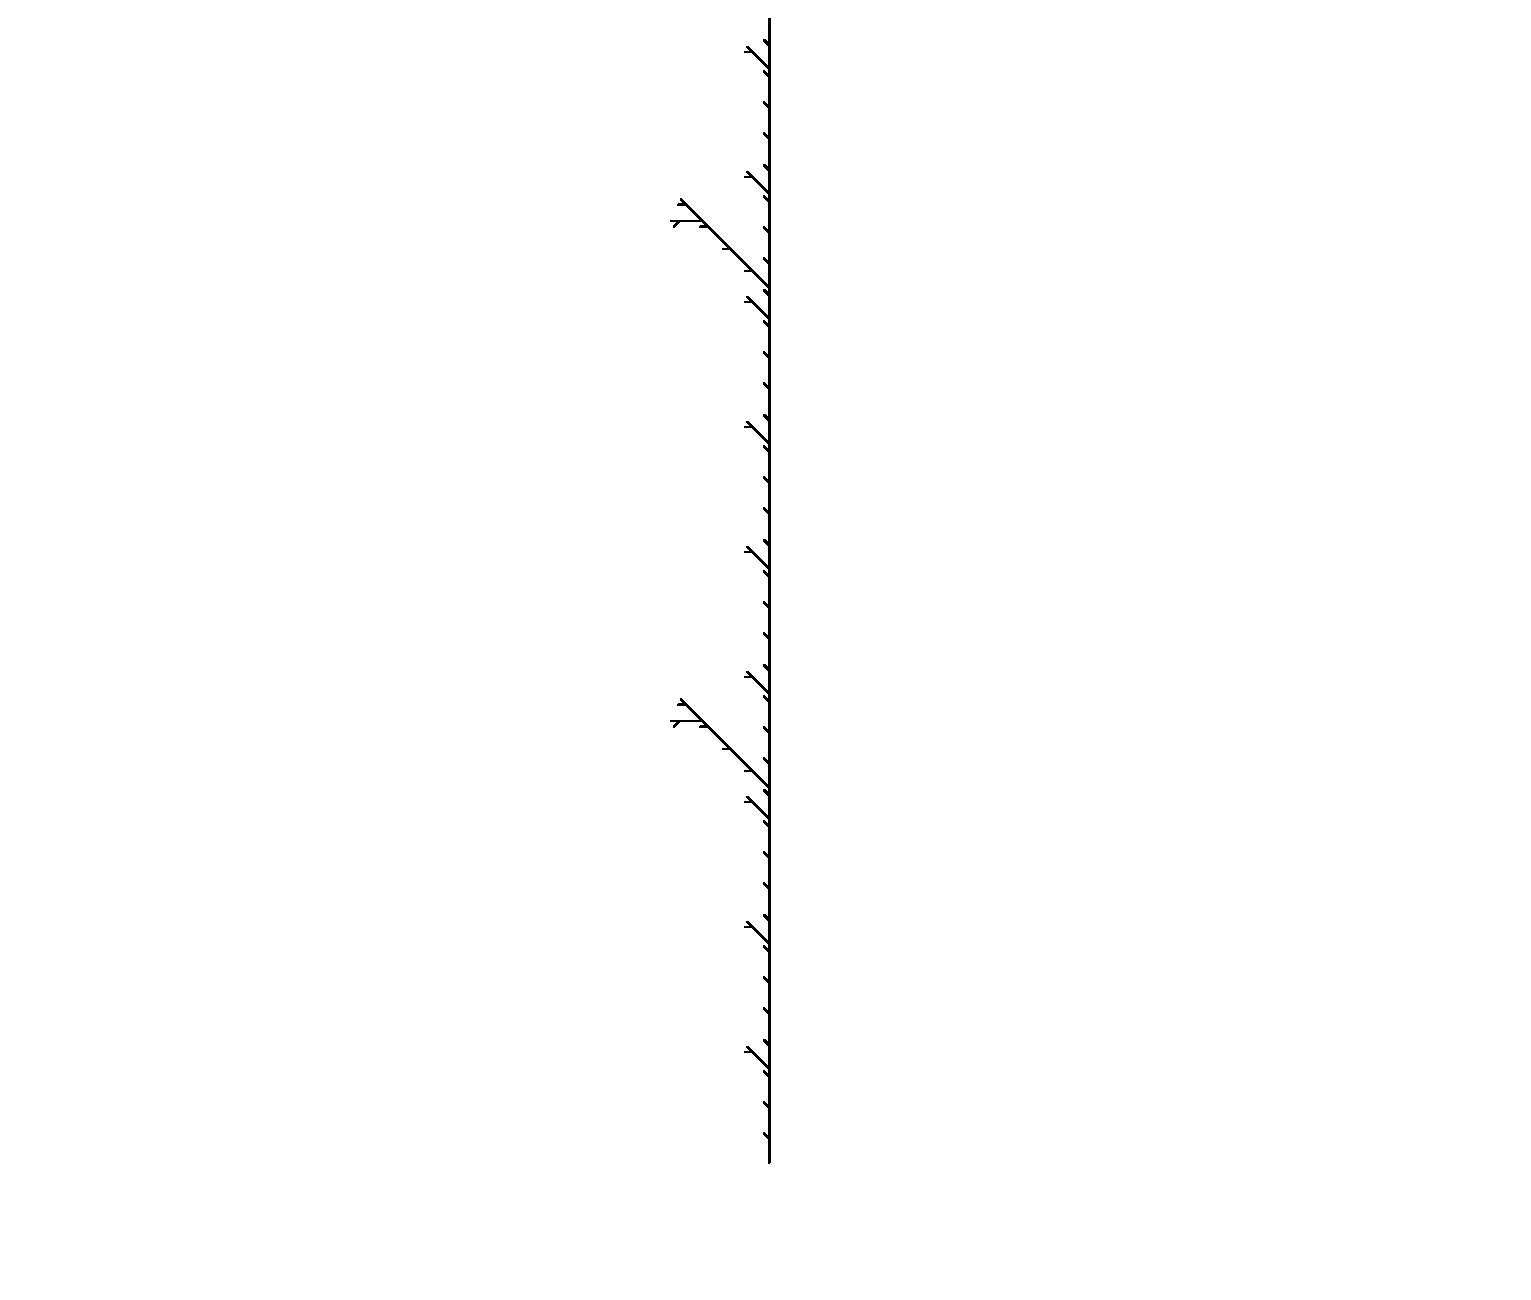
\includegraphics[width=.5\textwidth]{LSystem/plant_4} \\
Symmetrical F only & Symmetrical F only with +/- swapping
\end{tabular}

\begin{tabular}{ c c }
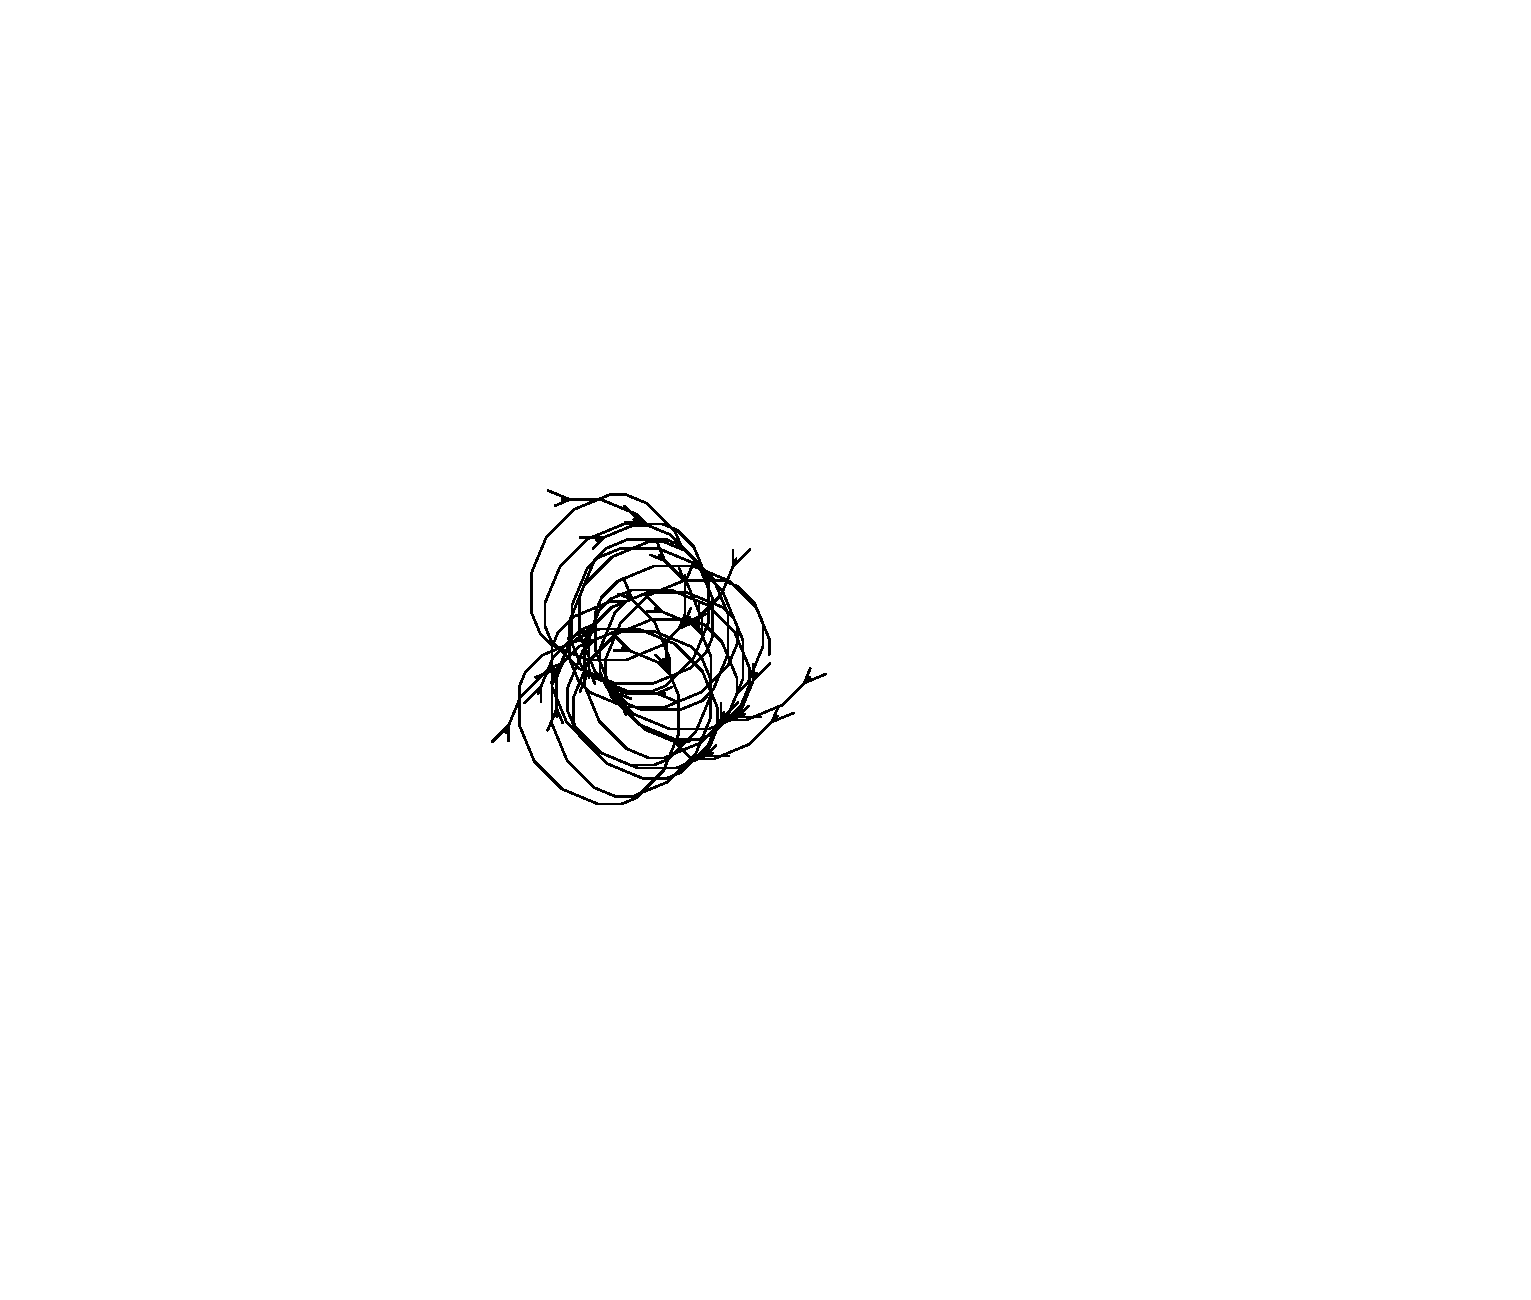
\includegraphics[width=.5\textwidth]{LSystem/plant_5} &

\includegraphics[width=.5\textwidth]{LSystem/plant_6} \\
Turning F & Symmetrical Turning F \\

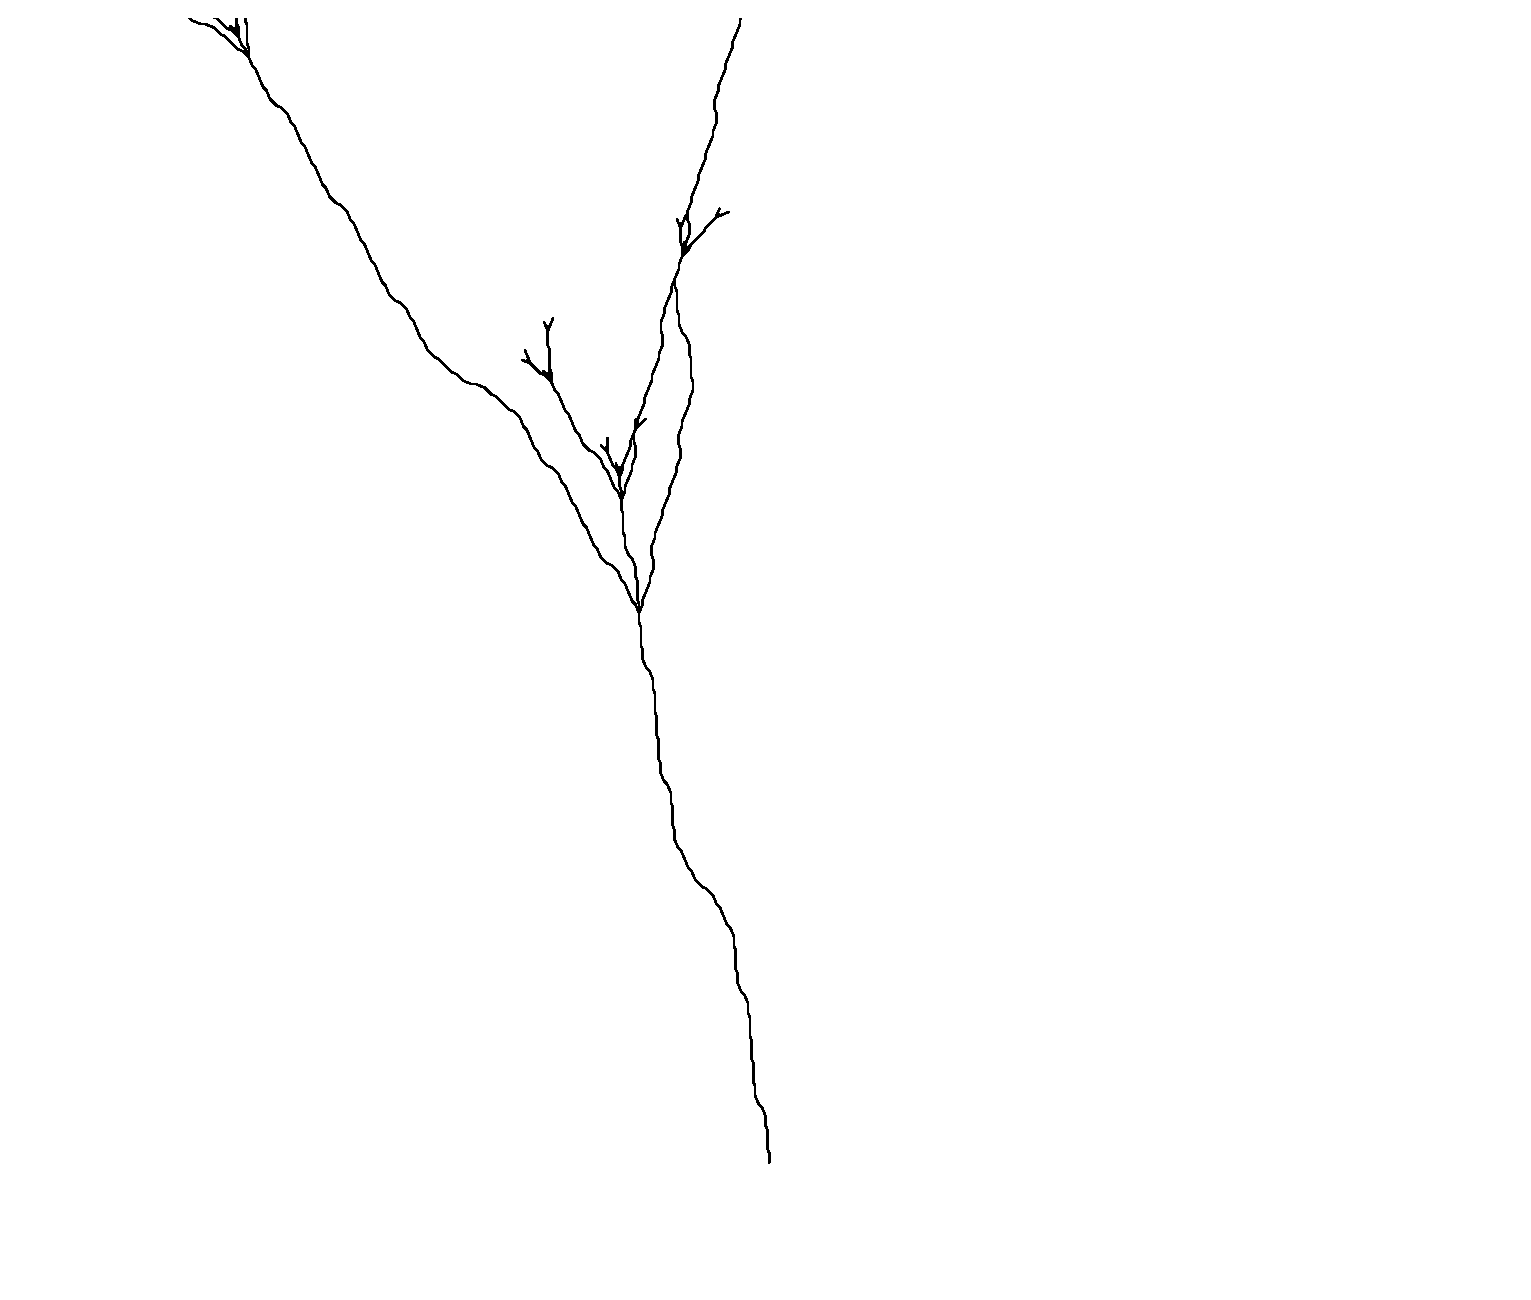
\includegraphics[width=.5\textwidth]{LSystem/plant_7} &
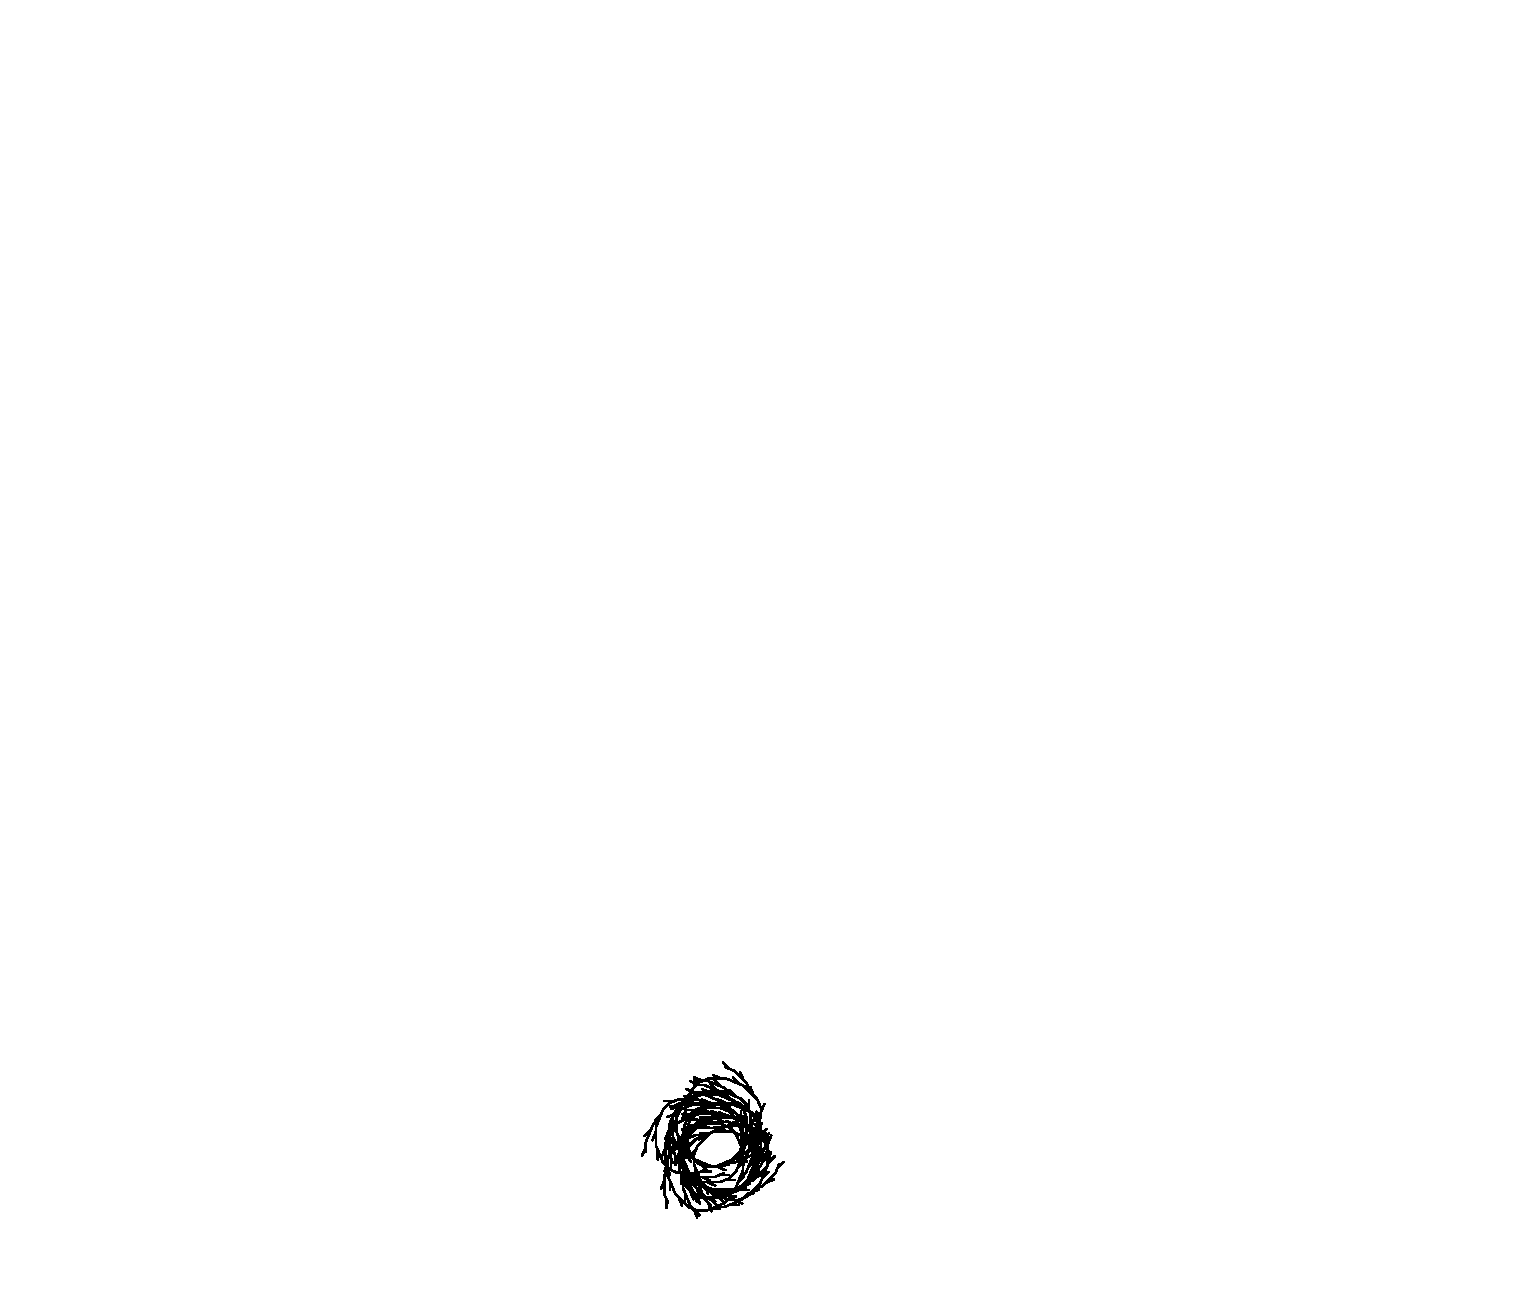
\includegraphics[width=.5\textwidth]{LSystem/plant_8} \\
Symmetrical Turning F with +/- swapping & Similar G \& F
\end{tabular}

\begin{tabular}{ c c c }
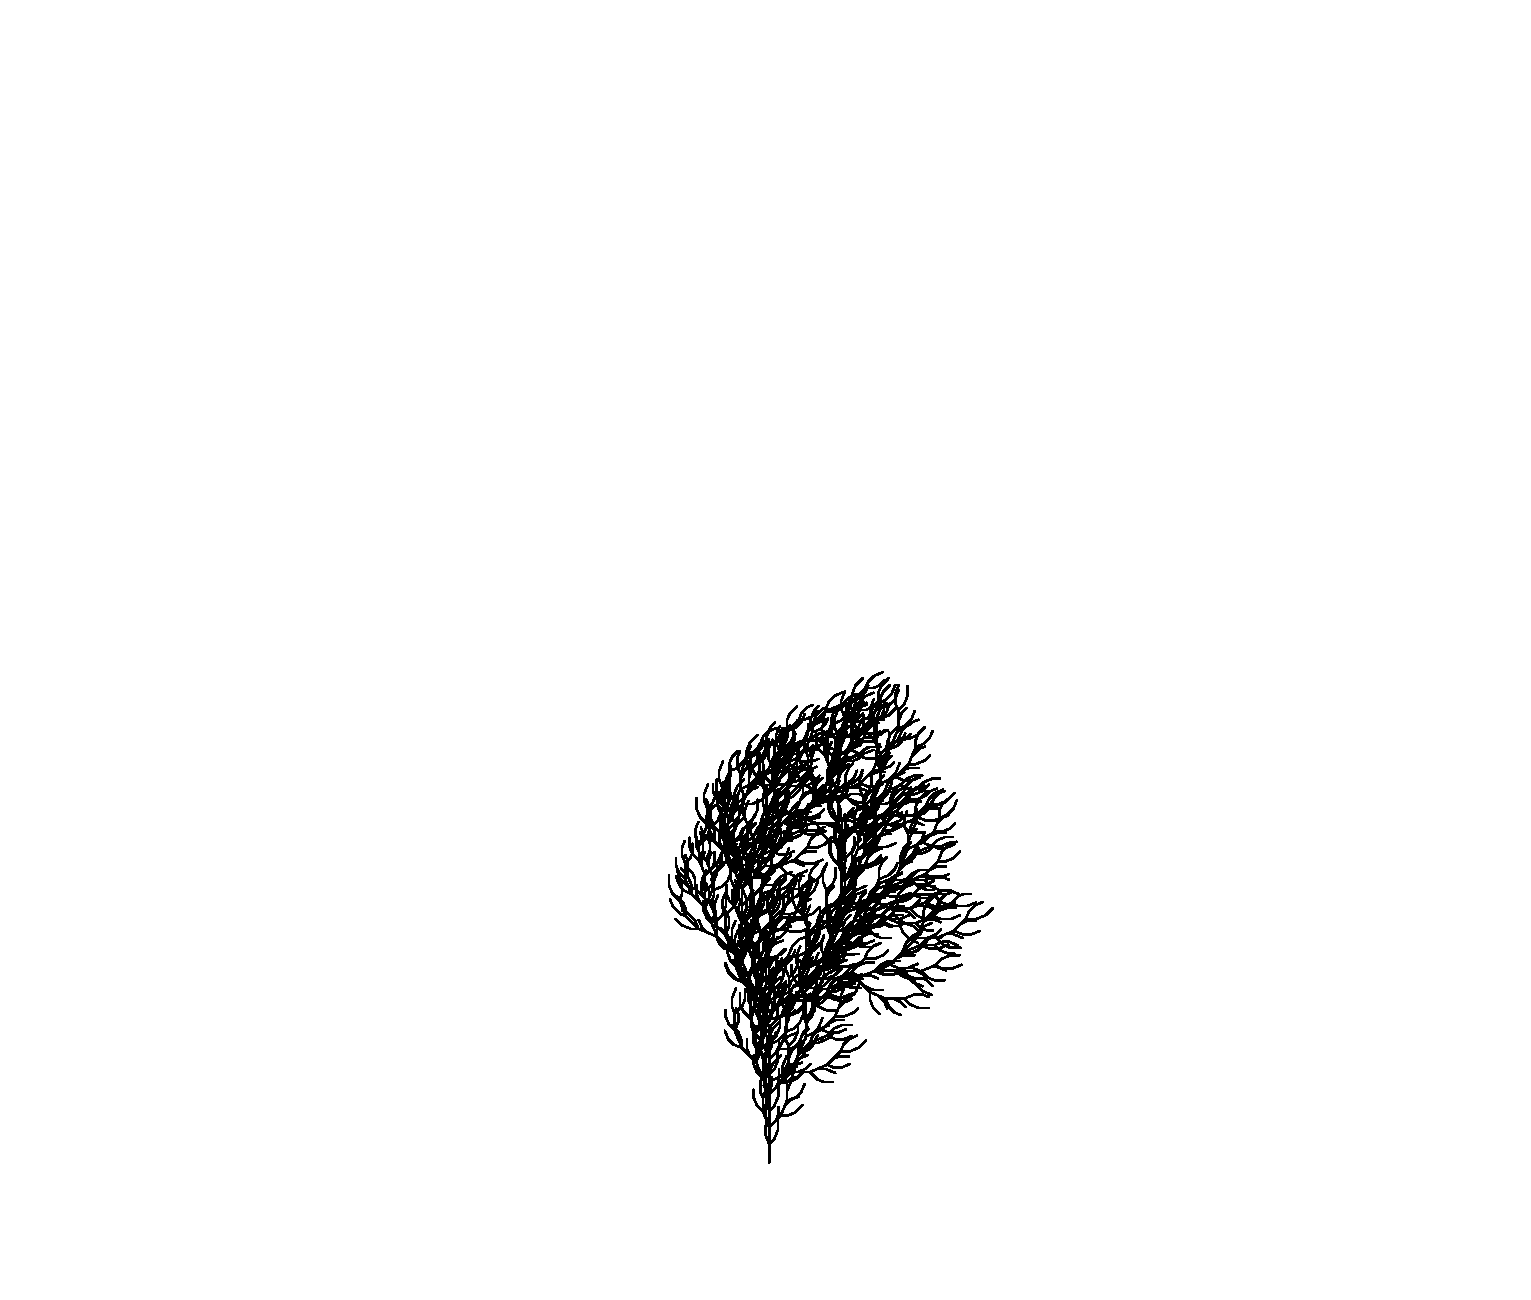
\includegraphics[width=.3\textwidth]{LSystem/plant_9} &
\includegraphics[width=.3\textwidth]{LSystem/lsystem_b} &
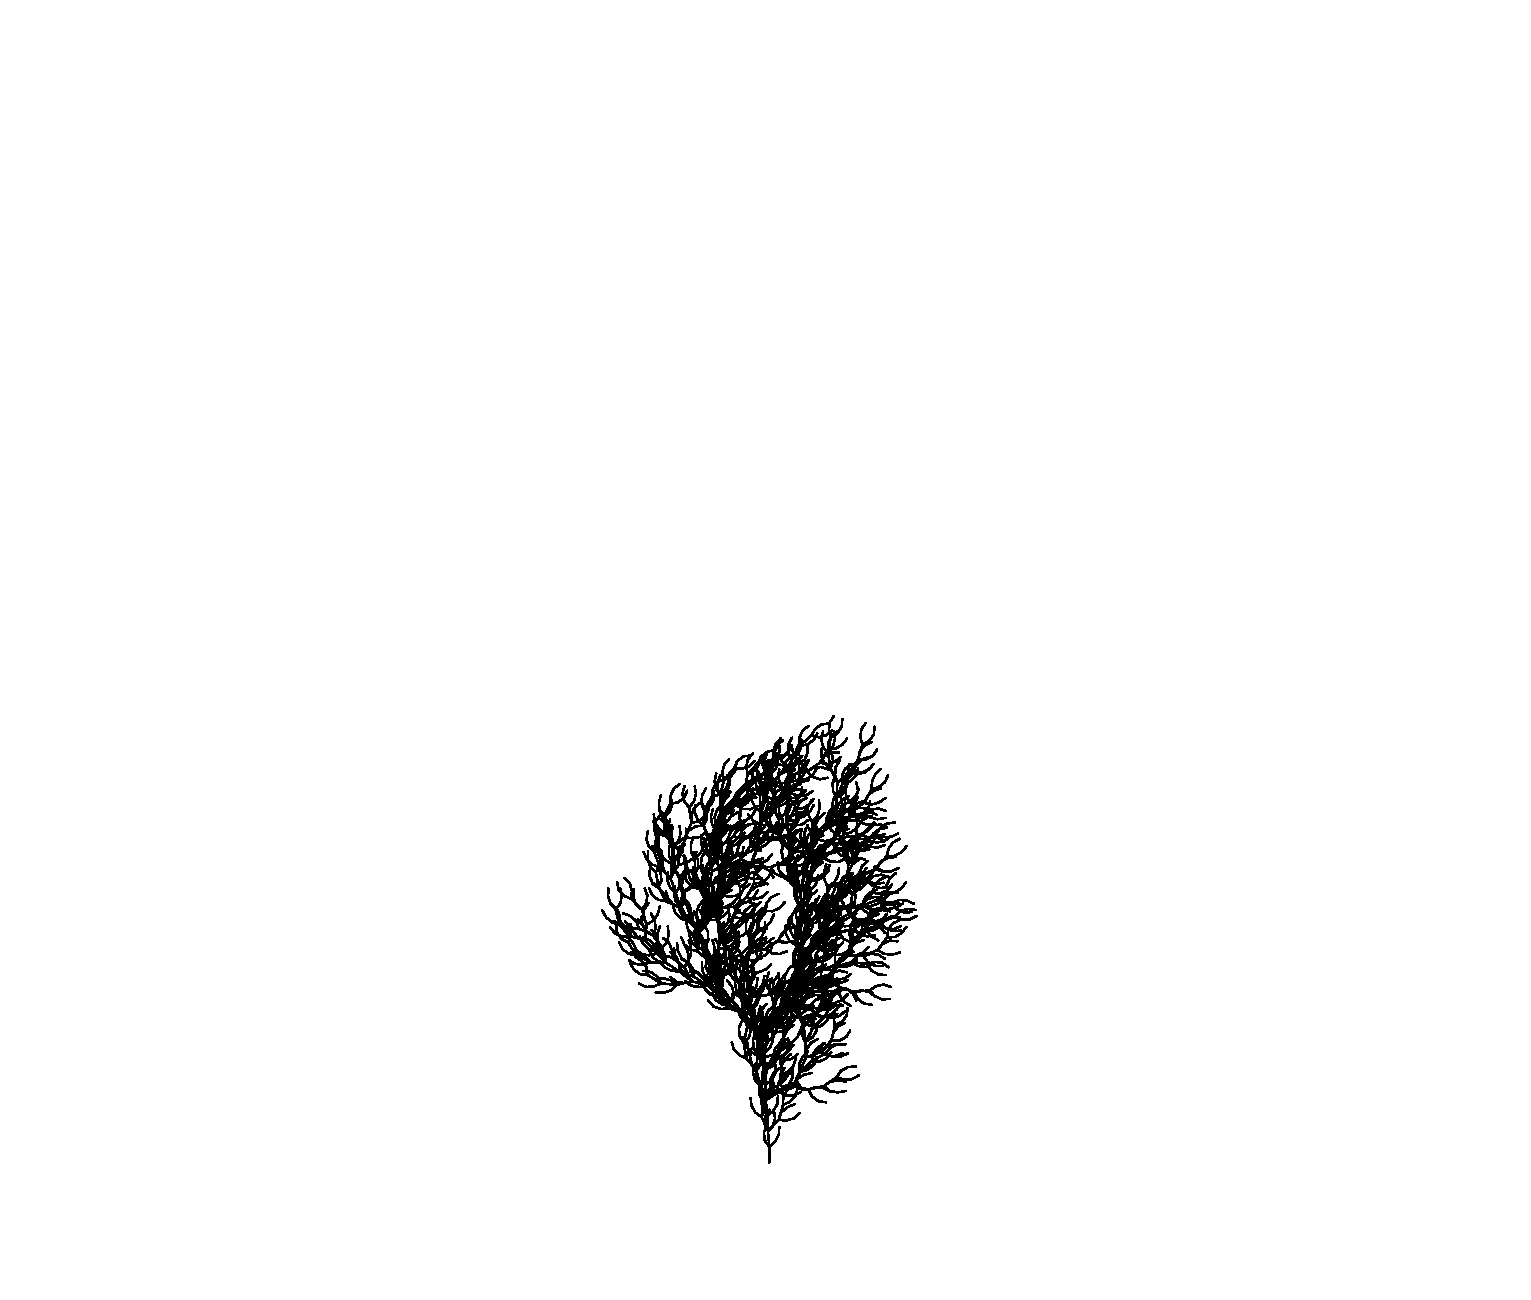
\includegraphics[width=.3\textwidth]{LSystem/plant_10} \\
Randomized distance (d) & 7.24(b) for comparison & Randomized turn ($\delta$)
\end{tabular}

\newpage
\section{RIFS Results} \label{RIFS_results}
\begin{tabular}{ c c }
\includegraphics[width=.5\textwidth]{RIFS/rifs_sierpinski} &
\includegraphics[width=.5\textwidth]{RIFS/rifs_square} \\
Sierpinski Gasket & Square \\
\includegraphics[width=.5\textwidth]{RIFS/rifs_barnsleyfern} &
\includegraphics[width=.5\textwidth]{RIFS/rifs_tree} \\
Barnsley Fern\footnote{I'm pretty sure the one in the book was rotated after it was generated to make it look more like a fern.} & Tree
\end{tabular}

\chapter{Code}
Insert code here.   You can use the listing environment or use doxygen.



% chapters in backmatter don't have numbers, but they appear in the
% table of contents, and are numbered BM-X where X is the page number
% relative to where the backmatter begins.
% \backmatter


\end{document}
